% Cross-view association (Online Methods) -- STANDALONE copy of the manuscript
% subsection, split out on instruction (Eric, 2026-08-26: "give me a tex file
% with the changes"). Two changes against the version in luc3d.tex:
%
%   1. RE-LETTERED for the current Figure 3. The old text pointed at the
%      pre-renumbering panels -- C for grouping accuracy, D for the ratio
%      sweep, E for time per frame. Figure 3 now runs A grouping strategies,
%      B hypotheses per frame, C one grouping hypothesis, D an identity switch,
%      E grouping accuracy, F time per frame, G/H the ratio sweep, so those
%      three references move to E, G/H and F respectively.
%   2. SHORTENED from ~1,250 words to ~700. Cut were the cap-removal history,
%      the skipped-frame arithmetic (a subtraction the reader can do), the
%      restated ground-truth-coverage sentence, the two-pass framing of the
%      ablation, and the self-justifying asides. Every number that appears on
%      the artwork or in a caption is retained.
%
% The body below is identical to figures/drafts/new_luc3d.tex's
% \subsection{Cross-view association}. The two figures are included only so the
% \ref{fig3} / \ref{fig6} calls resolve; their captions here are stubs, and the
% real captions live in the manuscript.
%
%   pdflatex methods_cross_view_association.tex     (from figs/figures/drafts/)
\documentclass[11pt]{article}
\usepackage[margin=2.5cm]{geometry}
\usepackage{graphicx}
\usepackage{amsmath}
\usepackage[numbers]{natbib}
\begin{document}

\section*{Online Methods}

\subsection*{Cross-view association}\label{methods-association-standalone}

For each frame the application maintains a set of 3D targets and solves one Hungarian assignment per camera, committing each camera's assignment before the next camera is solved, at a cost of $O(C \cdot A^3)$ for $A$ animals and $C$ cameras. The cost of pairing a target $t$ with a detection $d$ is summed over the skeleton nodes $k$ with per-node weights $w_k$, where a weight of zero removes that node, and is negated so that the solver minimizes it (\texttt{pose/cross-view-tracker.js}). The two-dimensional term compares the detection with the target's projection $\pi(t)$ into that camera, in undistorted ideal-pinhole coordinates,
\[
  w_k \cdot corr2d \cdot \left(1 - \frac{|d_k - \pi(t)_k|}{velThresh \cdot (1 + \Delta t)}\right) \cdot e^{-\lambda \Delta t}
\]
where $\Delta t$ is the target's age and $\lambda$ the time penalty, so age both widens the distance allowance and decays the whole term. The three-dimensional term is on the perpendicular distance from the target's 3D point to the ray back-projected from the detection, with no age decay,
\[
  w_k \cdot corr3d \cdot \left(1 - \frac{dist(t_k, ray(d_k))}{distThresh}\right)
\]
Both thresholds are soft, so exceeding one drives its term negative rather than preventing the pairing. The previous default is $corr2d = 1$ and $corr3d = 6$ (the ratio $r = 6$ marked in Figures~\ref{fig3}G and H), with velocityThreshold 10, distanceThreshold 50 and timePenalty 0.1. The shipped fresh-anchor configuration, drawn in Figures~\ref{fig3}E, G, H and~\ref{fig6}A, is the same tracker with per-view detections older than 20 frames expiring from the 3D anchor, the anchor updated synchronously, and the 3D normalizer 25 rather than 50.

The method compared against is our reimplementation of the per-frame procedure of \citep{Maree2024}, which enumerates all $(A!)^C$ groupings of a frame's detections into identities, triangulates and reprojects each, and keeps the lowest-error grouping, hereafter exhaustive enumeration. It is undefined unless every camera holds exactly $A$ detections, so only such frames were eligible and ineligible frames were counted rather than dropped. The benchmark covers the 92 multi-animal sessions carrying both pool detections and proofread ground truth, 50 of the 56 Mouse-Dyad-10M sessions and the 42 multi-animal SLAP-2M sessions, of which 4,591,864 of 9,678,503 frames were eligible and every one was computed, the three- and four-animal configurations at a measured 2.7 and 5.5 seconds per frame against 11 to 16 milliseconds for two animals. Four animals in six cameras exceeds the harness's cap of one million hypotheses per frame by a factor of 191 and was not run, so its cost in Figure~\ref{fig3}F is an arithmetic bound drawn with an open marker, taking the $(A!)^{(C-1)} = 7{,}962{,}624$ hypotheses that remain once the global relabeling symmetry is removed at the cheapest rate measured anywhere in the sweep, 249 microseconds each, and running up to the as-published $(A!)^C$ at the 396 microseconds measured in the largest configuration that did run.

Grouping quality in Figure~\ref{fig3}E compares partitions rather than labels, so a consistent relabeling of identities is not counted as an error; 4,591,725 of the computed frames carry a transferred ground-truth match and are scored. Two conventions separate the arms. Exhaustive enumeration has no cross-frame identity of its own, so the harness threads identity between consecutive computed frames by nearest-3D-centroid matching to make its identity metrics computable at all, which is scaffolding rather than part of the published method, leaving the per-frame agreement rate as the like-for-like comparison. And the arms are scored over different exposures, exhaustive enumeration over the 21,622,345 clean camera-frames it computed and the greedy arms over whole sessions, 45,021,960 camera-frames, so each rate is labeled with its own denominator.

The sweep in Figures~\ref{fig3}G and H fixes $corr2d = 1$ and samples twelve ratios over all 50 Mouse-Dyad-10M sessions at full length, for the fresh-anchor configuration drawn against the exhaustive reference and for the previous default, which is deposited. Only the ratio matters, verified on an earlier 24-cell grid over eight sessions where every pair of cells sharing a ratio returned identical IDF1 and identical switch counts, which is why the panels plot it. Switches are reported per 100,000 camera-frames because a total is uninterpretable without its denominator; that denominator is taken per camera and session from the scorer's own frame counts and is checked identical between the arms before they are drawn on one axis.

% ---- The two referenced figures, included so \ref resolves. Stub captions;
% the manuscript carries the real ones.
\setcounter{figure}{2}
\begin{figure}[!htb]
  \centering
  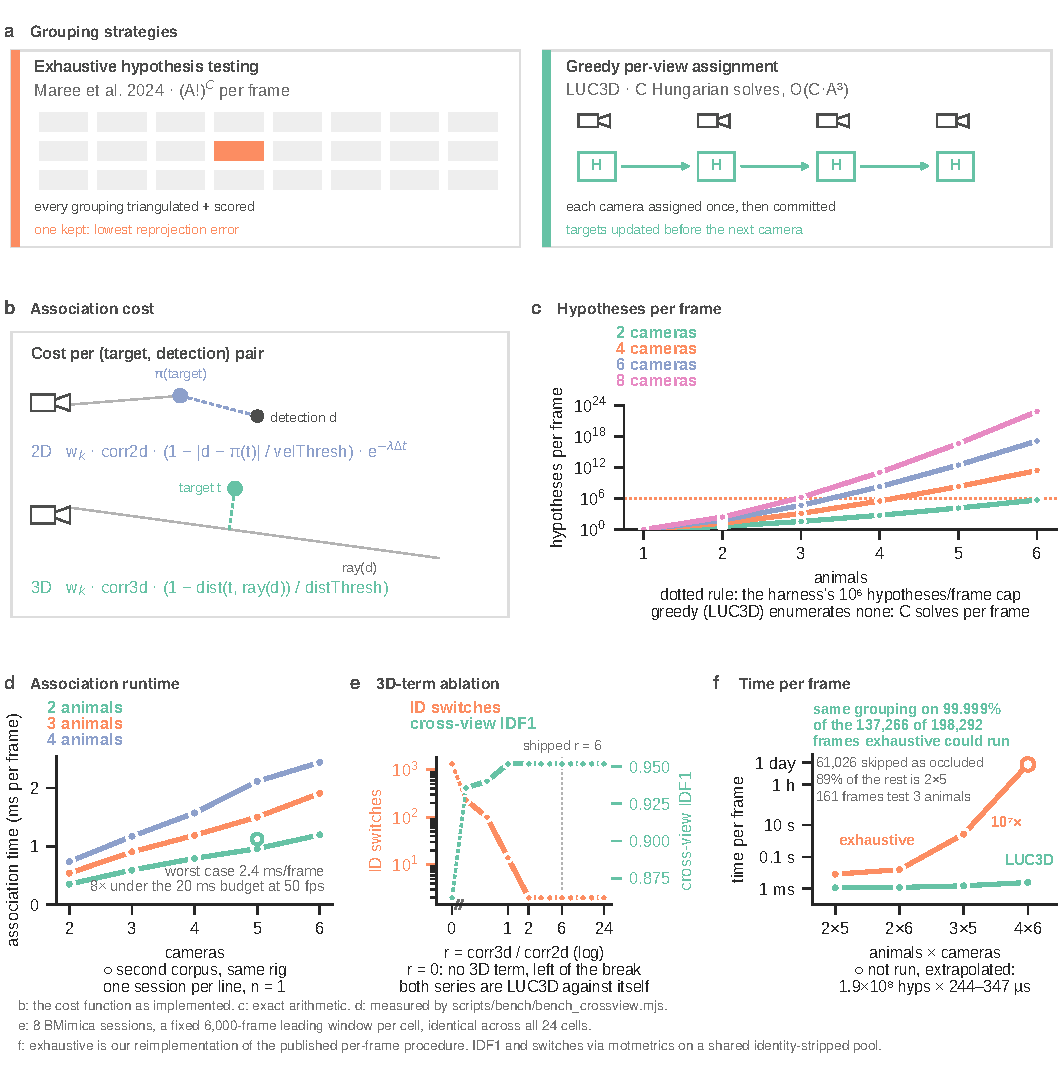
\includegraphics[width=1\textwidth]{../fig3/fig3.pdf}
  \caption{\textbf{Cross-view tracking algorithm} (stub caption, see the manuscript). \textbf{A}, Grouping strategies. \textbf{B}, Hypotheses per frame. \textbf{C}, One grouping hypothesis in two camera views. \textbf{D}, An identity switch in one camera view. \textbf{E}, Grouping accuracy. \textbf{F}, Time per frame. \textbf{G}, \textbf{H}, The 3D term's ratio sweep, switches and cross-view IDF1.}
  \label{fig3}
\end{figure}

\setcounter{figure}{5}
\begin{figure}[!htb]
  \centering
  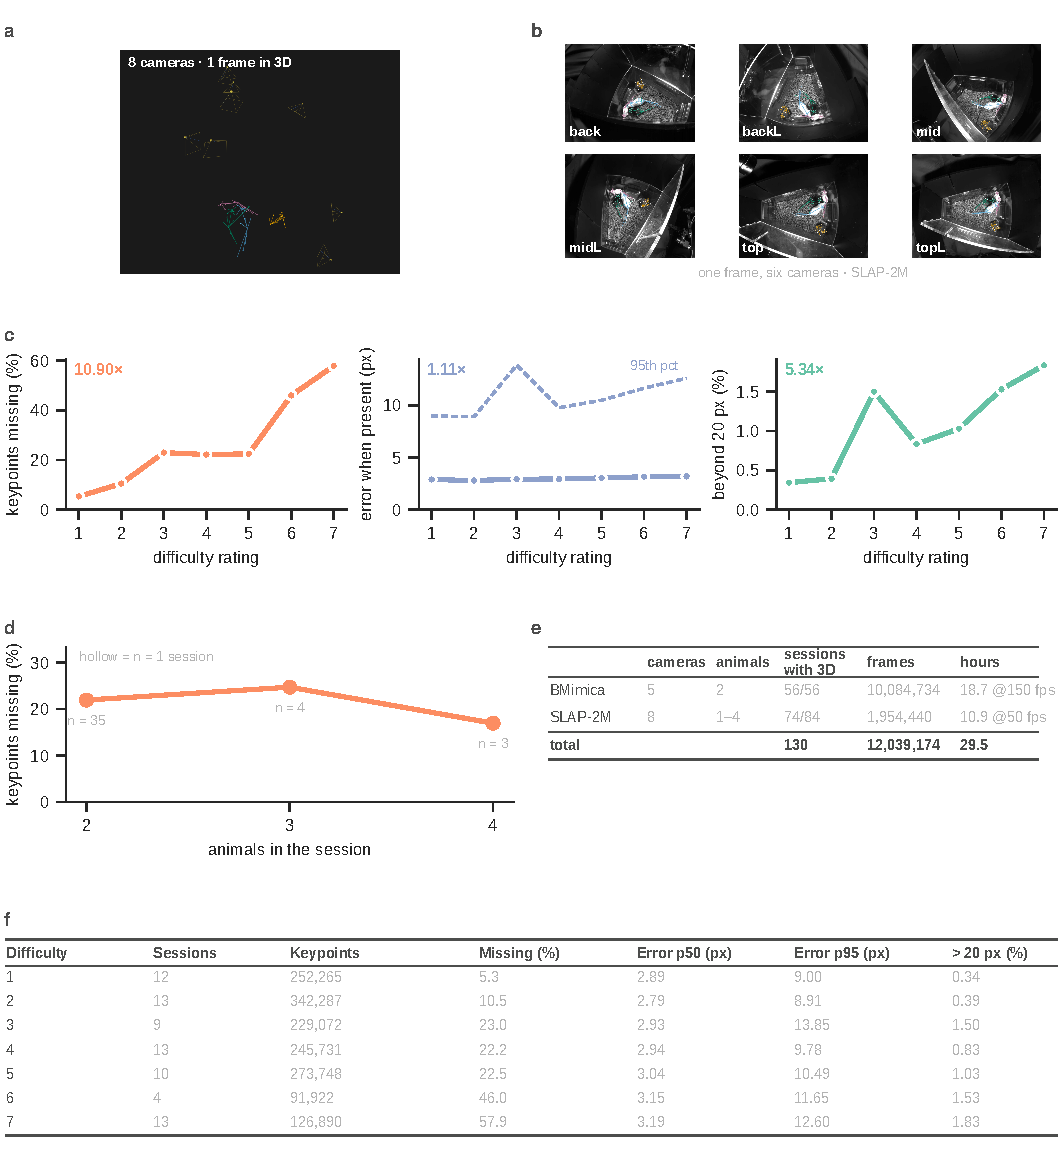
\includegraphics[width=1\textwidth]{../fig6/fig6.pdf}
  \caption{\textbf{Cross-view identity, and the fresh-anchor staleness horizon} (stub caption, see the manuscript). \textbf{A}, Within-view against cross-view IDF1. \textbf{B} to \textbf{D}, Per-session comparisons on SLAP-2M. \textbf{E}, The tracker's 2D and 3D anchor correspondence. \textbf{F}, The fresh-anchor parameter sweep.}
  \label{fig6}
\end{figure}

\begin{thebibliography}{9}
\bibitem{Maree2024} Maree, L., Afshar, S., Oline, S., Leonardis, E. J., Falkner, A. L., \& Pereira, T. D. (2024). Multi-view triangulation-enabled annotation for multi-animal 3D pose in SLEAP. In \textit{Measuring Behavior}.
\end{thebibliography}

\end{document}
